\documentclass{ximera}
\graphicspath{  %% When looking for images,
{./}            %% look here first,
{./pictures/}   %% then look for a pictures folder,
{../pictures/}  %% which may be a directory up.
{../../pictures/}  %% which may be a directory up.
{../../../pictures/}  %% which may be a directory up.
{../../../../pictures/}  %% which may be a directory up.
}

\usepackage{listings}
%\usepackage{circuitikz}
\usepackage{xcolor}
\usepackage{amsmath,amsthm}
\usepackage{subcaption}
\usepackage{graphicx}
\usepackage{tikz}
%\usepackage{tikz-3dplot}
\usepackage{amsfonts}
%\usepackage{mdframed} % For framing content
%\usepackage{tikz-cd}

  \renewcommand{\vector}[1]{\left\langle #1\right\rangle}
  \newcommand{\arrowvec}[1]{{\overset{\rightharpoonup}{#1}}}
  \newcommand{\ro}{\texttt{R}}%% row operation
  \newcommand{\dotp}{\bullet}%% dot product
  \renewcommand{\l}{\ell}
  \let\defaultAnswerFormat\answerFormatBoxed
  \usetikzlibrary{calc,bending}
  \tikzset{>=stealth}
  




%make a maroon color
\definecolor{maroon}{RGB}{128,0,0}
%make a dark blue color
\definecolor{darkblue}{RGB}{0,0,139}
%define the color fourier0 to be the maroon color
\definecolor{fourier0}{RGB}{128,0,0}
%define the color fourier1 to be the dark blue color
\definecolor{fourier1}{RGB}{0,0,139}
%define the color fourier 1t to be the light blue color
\definecolor{fourier1t}{RGB}{173,216,230}
%define the color fourier2 to be the dark green color
\definecolor{fourier2}{RGB}{0,100,0}
%define teh color fourier2t to be the light green color
\definecolor{fourier2t}{RGB}{144,238,144}
%define the color fourier3 to be the dark purple color
\definecolor{fourier3}{RGB}{128,0,128}
%define the color fourier3t to be the light purple color
\definecolor{fourier3t}{RGB}{221,160,221}
%define the color fourier0t to be the red color
\definecolor{fourier0t}{RGB}{255,0,0}
%define the color fourier4 to be the orange color
\definecolor{fourier4}{RGB}{255,165,0}
%define the color fourier4t to be the darker orange color
\definecolor{fourier4t}{RGB}{255,215,0}
%define the color fourier5 to be the yellow color
\definecolor{fourier5}{RGB}{255,255,0}
%define the color fourier5t to be the darker yellow color
\definecolor{fourier5t}{RGB}{255,255,100}
%define the color fourier6 to be the green color
\definecolor{fourier6}{RGB}{0,128,0}
%define the color fourier6t to be the darker green color
\definecolor{fourier6t}{RGB}{0,255,0}

%New commands for this doc for errors in copying
\newcommand{\eigenvar}{\lambda}
%\newcommand{\vect}[1]{\mathbf{#1}}
\renewcommand{\th}{^{\text{th}}}
\newcommand{\st}{^{\text{st}}}
\newcommand{\nd}{^{\text{nd}}}
\newcommand{\rd}{^{\text{rd}}}
\newcommand{\paren}[1]{\left(#1\right)}
\newcommand{\abs}[1]{\left|#1\right|}
\newcommand{\R}{\mathbb{R}}
\newcommand{\C}{\mathbb{C}}
\newcommand{\Hilb}{\mathbb{H}}
\newcommand{\qq}[1]{\text{#1}}
\newcommand{\Z}{\mathbb{Z}}
\newcommand{\N}{\mathbb{N}}
\newcommand{\q}[1]{\text{``#1''}}
%\newcommand{\mat}[1]{\begin{bmatrix}#1\end{bmatrix}}
\newcommand{\rref}{\text{reduced row echelon form}}
\newcommand{\ef}{\text{echelon form}}
\newcommand{\ohm}{\Omega}
\newcommand{\volt}{\text{V}}
\newcommand{\amp}{\text{A}}
\newcommand{\Seq}{\textbf{Seq}}
\newcommand{\Poly}{\textbf{P}}
\renewcommand{\quad}{\text{    }}
\newcommand{\roweq}{\simeq}
\newcommand{\rowop}{\simeq}
\newcommand{\rowswap}{\leftrightarrow}
\newcommand{\Mat}{\textbf{M}}
\newcommand{\Func}{\textbf{Func}}
\newcommand{\Hw}{\textbf{Hamming weight}}
\newcommand{\Hd}{\textbf{Hamming distance}}
\newcommand{\rank}{\text{rank}}
\newcommand{\longvect}[1]{\overrightarrow{#1}}
% Define the circled command
\newcommand{\circled}[1]{%
  \tikz[baseline=(char.base)]{
    \node[shape=circle,draw,inner sep=2pt,red,fill=red!20,text=black] (char) {#1};}%
}

% Define custom command \strikeh that just puts red text on the 2nd argument
\newcommand{\strikeh}[2]{\textcolor{red}{#2}}

% Define custom command \strikev that just puts red text on the 2nd argument
\newcommand{\strikev}[2]{\textcolor{red}{#2}}

%more new commands for this doc for errors in copying
\newcommand{\SI}{\text{SI}}
\newcommand{\kg}{\text{kg}}
\newcommand{\m}{\text{m}}
\newcommand{\s}{\text{s}}
\newcommand{\norm}[1]{\left\|#1\right\|}
\newcommand{\col}{\text{col}}
\newcommand{\sspan}{\text{span}}
\newcommand{\proj}{\text{proj}}
\newcommand{\set}[1]{\left\{#1\right\}}
\newcommand{\degC}{^\circ\text{C}}
\newcommand{\centroid}[1]{\overline{#1}}
\newcommand{\dotprod}{\boldsymbol{\cdot}}
%\newcommand{\coord}[1]{\begin{bmatrix}#1\end{bmatrix}}
\newcommand{\iprod}[1]{\langle #1 \rangle}
\newcommand{\adjoint}{^{*}}
\newcommand{\conjugate}[1]{\overline{#1}}
\newcommand{\eigenvarA}{\lambda}
\newcommand{\eigenvarB}{\mu}
\newcommand{\orth}{\perp}
\newcommand{\bigbracket}[1]{\left[#1\right]}
\newcommand{\textiff}{\text{ if and only if }}
\newcommand{\adj}{\text{adj}}
\newcommand{\ijth}{\emph{ij}^\text{th}}
\newcommand{\minor}[2]{M_{#2}}
\newcommand{\cofactor}{\text{C}}
\newcommand{\shift}{\textbf{shift}}
\newcommand{\startmat}[1]{
  \left[\begin{array}{#1}
}
\newcommand{\stopmat}{\end{array}\right]}
%a command to give a name to explorations and hints and theorems
\newcommand{\name}[1]{\begin{centering}\textbf{#1}\end{centering}}
\newcommand{\vect}[1]{\vec{#1}}
\newcommand{\dfn}[1]{\textbf{#1}}
\newcommand{\transpose}{\mathsf{T}}
\newcommand{\mtlb}[2][black]{\texttt{\textcolor{#1}{#2}}}
\newcommand{\RR}{\mathbb{R}} % Real numbers
\newcommand{\id}{\text{id}}
\newcommand{\coord}[1]{\langle#1\rangle}
\newcommand{\RREF}{\text{RREF}}
\newcommand{\Null}{\text{Null}}
\newcommand{\Nullity}{\text{Nullity}}
\newcommand{\Rank}{\text{Rank}}
\newcommand{\Col}{\text{Col}}
\newcommand{\Ef}{\text{EF}}
\newcommand{\boxprod}[3]{\abs{(#1\times#2)\cdot#3}}

\author{Zack Reed}
%borrowed from selinger linear algebra
\title{Vector Subspaces: Lines and Planes}
\begin{document}
\begin{abstract}


\end{abstract}
\maketitle



\section{Planes}
\label{sec:planes}

As promised, we also find better ways to discuss planes and hyperplanes, in accordance with the ideas of normal vectors and the dot product.

First, much like with lines we can extend the notion of planes as $2D$ spans into a vector equation. 

Consider a point $P$ and two direction
vectors $\vect{d}$ and $\vect{e}$ that are not parallel to each
other. 

If $\vec{p}$ is the vector going from the origin to $P$, then any vector $\vec{q}$ on the plane is the result of adding $\vec{p}$ to a linear combination of the direction vectors $\vec{e}$ and $\vec{d}$.

\begin{center}
  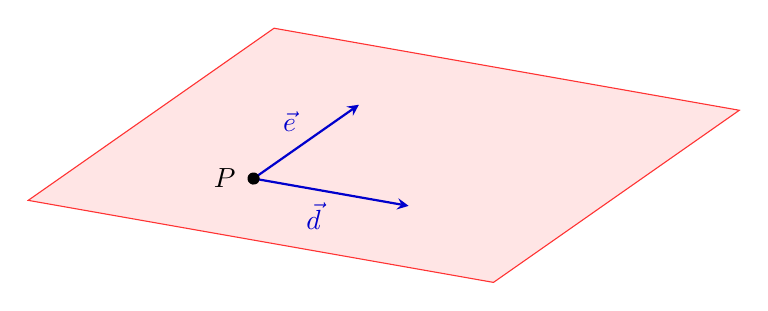
\begin{tikzpicture}[rotate=-10]
    \filldraw[draw=red!80,fill=red!10](-2,0,-5) -- (4,0,-5) -- (4,0,2) -- (-2,0,2) -- cycle;
    \draw[->,thick,blue!80!black](0,0,0) -- node[below left] {$\vect{d}$} (2,0,0);
    \draw[->,thick,blue!80!black](0,0,0) -- node[above left] {$\vect{e}$} (0,0,-3);
    \fill (0,0) circle [radius=2.2pt] node [left=3pt] {$P$};
  \end{tikzpicture}
\end{center}

This brings us to the following definition: 


\begin{definition}\name{Vector equation of a plane}\label{def:vector-equation-of-plane}

  Let $\vect{p}$ be a vector and let $\vect{d},\vect{e}$ be non-zero,
  non-parallel vectors. Then
  \begin{equation*}
    \vect{q} = \vect{p} + t\,\vect{d} + s\,\vect{e}
  \end{equation*}
  is the \textbf{vector equation} of the plane offset by $\vec{p}$ and spanned by $\vec{d}$ and $\vec{e}$.
\end{definition}

The vector equation of a plane can also be written in
\textbf{component form}

\begin{equation*}
  \startmat{c} x_1 \\ x_2 \\ \vdots \\ x_n \stopmat
  = \startmat{c} p_1 \\ p_2 \\ \vdots \\ p_n \stopmat
  + t \startmat{r} d_1 \\ d_2 \\ \vdots \\ d_n \stopmat,
  + s \startmat{r} e_1 \\ e_2 \\ \vdots \\ e_n \stopmat.
\end{equation*}

\begin{example}\name{Vector and parametric equations}\label{ex:plane-from-three-points}
  Find the plane through the
  points $P = (1,2,0,0)$, $Q = (2,2,0,1)$, and $R = (0,1,1,0)$.
\end{example}

\begin{solution}
  We can use $P$ as the base point and $\longvect{PQ}$ and
  $\longvect{PR}$ as the direction vectors. We have
  \begin{equation*}
    \longvect{PQ} =
    \startmat{c} 2\\2\\0\\1 \stopmat
    - \startmat{c} 1\\2\\0\\0 \stopmat
    = \startmat{c} 1\\0\\0\\1 \stopmat
    \quad\mbox{and}\quad
    \longvect{PR} =
    \startmat{c} 0\\1\\1\\0 \stopmat
    - \startmat{c} 1\\2\\0\\0 \stopmat
    = \startmat{c} -1\\-1\\1\\0 \stopmat.
  \end{equation*}

  Therefore the vector equation is

  \begin{equation*}
    \startmat{c} x\\y\\z\\w \stopmat
    = \startmat{c} \answer{1}\\\answer{2}\\\answer{0}\\\answer{0} \stopmat
    + t\,\startmat{c} \answer{1}\\\answer{0}\\\answer{0}\\\answer{1} \stopmat
    + s\,\startmat{c} \answer{-1}\\\answer{-1}\\\answer{1}\\\answer{0} \stopmat.
\end{equation*}
\end{solution}

In the special case of 3 dimensions, a plane can also be described by
a point and a normal vector, $\vec{n}$. This leverages the strategy hinted at in the previous section, where we determined whether a point was on a line by checking orthogonality with a vector $\vec{n}$ that was orthogonal to the line's direction vector.

In $\RR^3$ in particular, planes take up $2$ out of $3$ dimensions in the space, and so it is often more efficient and at times very beneficial to describe planes using only a single vector $\vec{n}$, rather than the two direction vectors. This kind of strategy comes up quite often in engineering and the sciences, and if you've taken vector calculus this idea should be familiar to you.

First, a \textbf{normal vector} of a plane is a vector that is
perpendicular to the plane.
\begin{center}
  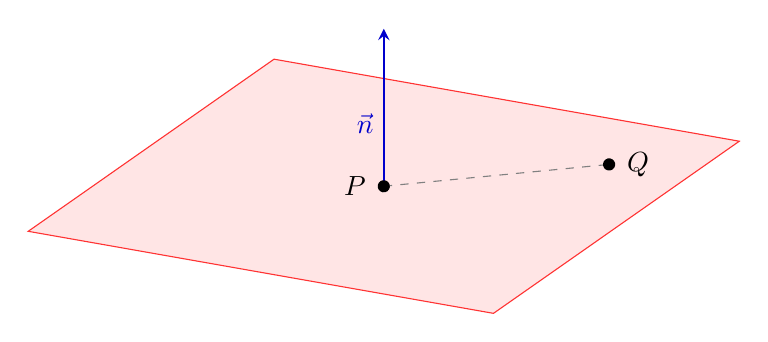
\begin{tikzpicture}[rotate=-10]
    \filldraw[draw=red!80,fill=red!10](-3,0,-3.5) -- (3,0,-3.5) -- (3,0,3.5) -- (-3,0,3.5) -- cycle;
    \draw[->,thick,blue!80!black](0,0,0) -- node[left, pos=0.4] {$\vect{n}$} (100:2);
    \draw[dashed,gray](0,0,0) -- (2,0,-2);
    \fill (0,0,0) circle [radius=2.2pt] node [left=3pt] {$P$};
    \fill (2,0,-2) circle [radius=2.2pt] node [right=3pt] {$Q$};
  \end{tikzpicture}
\end{center}

Given a non-zero vector $\vect{n}$ in $\R^3$ and a point $P$, there
exists a unique plane that contains $P$ and has $\vect{n}$ as a normal
vector. This is because, again, the plane takes up $2/3$ of the dimensions of $\RR^3$, meaning that the rest of $\RR^3$ is characterized only by variation along a single remaining axis. While any vector not on the plane will suffice, only one vector $\vec{n}$ (or its negative) will be orthogonal to the plane. Hence, normal vectors allow us to strategically characterize planes succinctly.

To visualize this phenomenon, again create an orthonormal basis of $\RR^3$ using the following GeoGebra applet, but attend to the constraining of the final vector to a single direction (or its negative) to maintain the orthogonality.

\begin{center}
  \geogebra{ym8uzusc}{859}{457}
\end{center}


We wish to find an equation for this plane. The key feature of the normal vector is that it is orthogonal to any vector spanned by the plane's direction vectors $\vec{d}$ and $\vec{e}$. So, if any vector $\vec{q}$ is on the plane, then after un-shifting by $\vec{p}$ we should have a vector orthogonal to $\vec{n}$. This gives us our nice succinct definition of the plane.


\begin{equation*}
  \vect{n} \dotprod (\vect{q}-\vect{p}) = 0,
\end{equation*}
or equivalently,
\begin{equation*}
  \vect{n} \dotprod \vect{q} = \vect{n} \dotprod \vect{p}.
\end{equation*}

This is called the \textbf{normal equation} of the plane. Note that in
this equation, $\vect{n}$ and $\vect{p}$ are given and fixed, whereas
$\vect{q}$ is a variable ranging over the position vectors of all
points on the plane.



\begin{definition}\name{Normal equation of a plane in $\R^3$}\label{def:normal-equation-plane}

  Let $\vect{n}$ be a non-zero vector in $\R^3$, and let $P$ be a
  point with position vector $\vect{p}$. Then there is a unique plane through
  $P$ with normal vector $\vect{n}$. It is described by the equation
  \begin{equation*}
    \vect{n} \dotprod (\vec{p}-\vect{q}) = 0.
  \end{equation*}
  This equation is called the \textbf{normal equation} of the plane.
\end{definition}

\begin{example}\name{Finding the normal equation of a plane}\label{ex:normal-equation}

  Find the normal equation of the plane through the point $P=(1,3,0)$
  and orthogonal to $\vect{n}=\startmat{c}2\\1\\1\stopmat$.
\end{example}

\begin{solution}
  Let $\vect{p}=\startmat{c}1\\3\\0\stopmat$ be the position vector of $P$, and let
  $\vect{q}=\startmat{c}x\\y\\z\stopmat$ be the position vector of some arbitrary
  point $Q$ in the plane. 
  
  The normal equation is
  $\vect{n} \dotprod (\vec{q}-\vect{p}) = 0.$, which we
  can write in component form:

  \begin{equation*}
    \startmat{c}\answer{2}\\\answer{1}\\\answer{1}\stopmat
    \dotprod
    \startmat{c}x-\answer{1}\\y-\answer{3}\\z-\answer{0}\stopmat
    =0.
  \end{equation*}

  If we take the other form of the normal equation 
  
  $$vect{n} \dotprod \vect{q} = \vect{n} \dotprod \vect{p},$$
  
  we can pre-compute the dot product on the right-hand side:
  $\vect{n} \dotprod \vect{p} = \answer{5}$. 
  
  Therefore, the
  normal equation can also be written as

  \begin{equation*}
    \startmat{c}\answer{2}\\\answer{1}\\\answer{1}\stopmat
    \dotprod
    \startmat{c}x\\y\\z\stopmat
    = \answer{5}.
  \end{equation*}
\end{solution}

Notice that the last equation in Example~\ref{ex:normal-equation} can
also be written in the form
\begin{equation*}
  2x + y + z = 5.
\end{equation*}

This last form is called the \textbf{standard equation} of the plane.

\begin{definition}{Standard equation of a plane in $\R^3$}{standard-equation-plane}
  Let $\vect{n} = \startmat{c}a,b,c\stopmat^T$ be the normal vector for a plane that
  contains the point $P = (x_0, y_0, z_0)$. The \textbf{standard
    equation}%
  \index{plane!standard equation}%
  \index{standard equation of a plane} of the plane is given by
  \begin{equation*}
    ax + by + cz = d,
  \end{equation*}
  where $a,b,c,d \in \R$ and $d = ax_0 + by_0 + cz_0$.
\end{definition}

This is often the first definition of a plane that you will see in a calculus textbook, but without motivating the definition through normal vectors and dot products it is often a mystery why we can or would write planes in this way (or, it leads to poor generalizations from lines).

\begin{example}\name{Normal and standard equations}\label{exa:normal-from-three-points}

  Find normal and standard equations for the plane through the points
  $P = (0,1,3)$, $Q=(2,-1,0)$, and $R=(1,2,2)$.
\end{example}

\begin{solution}
  We first need to find a normal vector for the plane. This need motivates the final concept of the chapter, the \emph{cross product}, which we will discuss in the next section. So $\ldots$ to be continued!

\end{solution}

\end{document}
  
  Since the
  normal vector must be perpendicular to the plane, it must be
  orthogonal to both $\longvect{PQ}$ and $\longvect{PR}$. We can
  therefore use the cross product to compute a normal vector for the
  plane:
  \begin{equation*}
    \vect{n}
    ~=~
    \longvect{PQ} \times \longvect{PR}
    ~=~
    \startmat{r} 2 \\ -2 \\ -3 \stopmat
    \times
    \startmat{r} 1 \\ 1 \\ -1 \stopmat
    ~=~
    \startmat{r} 5 \\ -1 \\ 4 \stopmat.
  \end{equation*}
  \begin{center}
    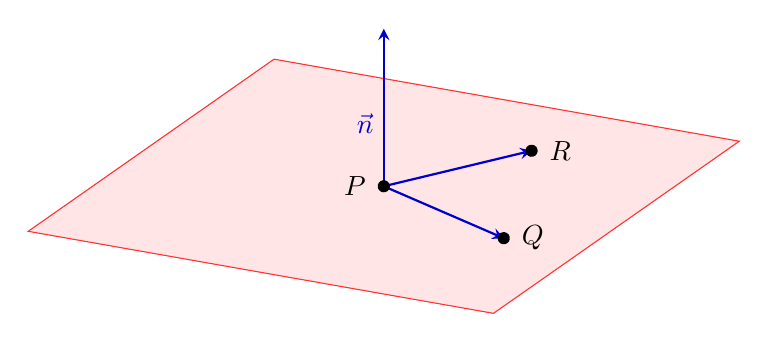
\begin{tikzpicture}[rotate=-10]
      \filldraw[draw=red!80,fill=red!10](-3,0,-3.5) -- (3,0,-3.5) -- (3,0,3.5) -- (-3,0,3.5) -- cycle;
      \draw[->,thick,blue!80!black](0,0,0) -- node[left, pos=0.4] {$\vect{n}$} (100:2);
      \draw[->,thick,blue!80!black](0,0,0) -- (2,0,1);
      \draw[->,thick,blue!80!black](0,0,0) -- (1,0,-2);
      \fill (0,0,0) circle [radius=2.2pt] node [left=3pt] {$P$};
      \fill (2,0,1) circle [radius=2.2pt] node [right=3pt] {$Q$};
      \fill (1,0,-2) circle [radius=2.2pt] node [right=3pt] {$R$};
    \end{tikzpicture}
  \end{center}
  Now we can easily obtain the normal equation from any point on the
  plane (say $P$) and the normal vector we just calculated:
  \begin{equation*}
    \startmat{r} 5 \\ -1 \\ 4 \stopmat
    \dotprod
    \startmat{r} x \\ y \\ z \stopmat
    =
    \startmat{r} 5 \\ -1 \\ 4 \stopmat
    \dotprod
    \startmat{r} 0 \\ 1 \\ 3 \stopmat
  \end{equation*}
  We get the standard equation by computing the dot products on the
  left- and right-hand sides:
  \begin{equation*}
    5x - y + 4z = 11.
  \end{equation*}
  It is worthwhile to double-check the answer by substituting each of
  the three original points $P$, $Q$, and $R$ into this equation.
  For example, for $Q=(2,-1,0)$, we obtain $5(2)-(-1)+4(0)$, which is
  indeed $11$.
\end{solution}

\begin{example}{Find the normal vector of a plane}{find-normal}
  Find a normal vector for the plane $2x+3y-z=7$.
\end{example}

\begin{solution}
  The standard equation $2x+3y-z=7$ can be rewritten as a normal
  equation
  \begin{equation*}
    \startmat{r} 2\\3\\-1 \stopmat
    \dotprod
    \startmat{c} x\\y\\z \stopmat
    = 7.
  \end{equation*}
  Therefore,
  \begin{equation*}
    \vect{n} = \startmat{r} 2\\3\\-1 \stopmat
  \end{equation*}
  is a normal vector for the plane.
\end{solution}


\begin{example}{Determine whether a point is on a plane}{point-plane-normal}
  Let $\vect{n} = \startmat{c}1,2,3\stopmat^T$ be the normal vector for a plane
  which contains the point $P = (2,1,4)$. Determine if the point
  $Q = (5,4,1)$ is in this plane.
\end{example}

\begin{solution}
  By Definition~\ref{def:normal-equation-plane}, $Q$ is a point in the
  plane if and only if
  \begin{equation*}
    \vect{n} \dotprod \vect{q} = \vect{n} \dotprod \vect{p},
  \end{equation*}
  where $\vect{p}$ and $\vect{q}$ are the position vectors of $P$ and
  $Q$, respectively.  Given $\vect{n}$, $P$, and $Q$ as above, this
  equation becomes
  \begin{equation*}
    \startmat{r} 1 \\ 2 \\ 3 \stopmat
    \dotprod
    \startmat{r} 5 \\ 4 \\ 1 \stopmat
    ~=~
    \startmat{r} 1 \\ 2 \\ 3 \stopmat
    \dotprod
    \startmat{r} 2 \\ 1 \\ 4 \stopmat.
  \end{equation*}
Since both sides of the equation are equal to $16$, the equation is
  true. So the point $Q$ is indeed in the plane determined by
  $\vect{n}$ and $P$.
\end{solution}

\begin{example}{Vector equation from normal equation}{vector-from-normal}
  Find a vector equation for the plane $x+3y-2z=7$.
\end{example}

\begin{solution}
  This is the same thing as finding the general solution of a system
  of one linear equation in 3 variables. Since there is only a single
  equation $x+3y-2z=7$, it is already in {\ef}. The variables
  $y$ and $z$ are free, so we set them equal to parameters: $z=t$ and
  $y=s$. The variable $x$ is a pivot variable, and we get
  $x=7+2t-3s$. So the general solution of the equation is
  \begin{equation*}
    \startmat{c} x\\y\\z \stopmat
    = \startmat{r} 7\\0\\0 \stopmat
    + t\,\startmat{r} 2\\0\\1 \stopmat
    + s\,\startmat{r} -3\\1\\0 \stopmat.
  \end{equation*}
  This is also a vector equation for the plane.
\end{solution}

\begin{example}{Intersection of two planes}{intersection-planes}
  Find the intersection of the planes $x-2y+z=0$ and
  $2x-3y-z=4$.%
  \index{intersection!of two planes}
\end{example}



\begin{solution}
  Finding the intersection means finding all of the points $(x,y,z)$
  that are on both planes simultaneously. This is the same as solving
  the system of equations
  \begin{eqnarray*}
    x-2y+z &=& 0, \\
    2x-3y-z &=& 4.
  \end{eqnarray*}
  We solve the system by Gauss-Jordan elimination:
  \begin{equation*}
    \startmat{ccc|c}
      1 & -2 & 1 & 0 \\
      2 & -3 & -1 & 4
    \stopmat
    \stackrel{R_2\rowop R_2-2R_1}{\roweq}
    \startmat{ccc|c}
      1 & -2 & 1 & 0 \\
      0 & 1 & -3 & 4
    \stopmat
    \stackrel{R_1\rowop R_1+2R_2}{\roweq}
    \startmat{ccc|c}
      1 & 0 & -5 & 8 \\
      0 & 1 & -3 & 4
    \stopmat.
  \end{equation*}
  Therefore, the general solution is
  \begin{equation*}
    \startmat{c} x\\y\\z \stopmat
    =
    \startmat{c} 8\\4\\0 \stopmat
    + t\,\startmat{c} 5\\3\\1 \stopmat,
  \end{equation*}
  where $t$ is a parameter. This is the parametric equation of a
  line. Therefore, the two planes intersect in a line. Specifically,
  the intersection is the line through the point $(8,4,0)$ with
  direction vector $\startmat{c}5,3,1\stopmat^T$.
\end{solution}

\begin{example}{Intersection of a line and a plane}{intersection-line-plane}
  Find the intersection of the line
  \begin{equation*}
    \startmat{r} x \\ y \\ z \stopmat
    = \startmat{r} 1 \\ 2 \\ 0 \stopmat
    + t \startmat{r} -1 \\ 1 \\ 2 \stopmat
  \end{equation*}
  and the plane $2x+2y-z = 2$.%
  \index{intersection!of a line and a plane}
\end{example}

\begin{solution}
  Let us write
  \begin{equation*}
    \vect{p}=\startmat{c}1\\2\\0\stopmat,
    \quad
    \vect{d}=\startmat{c}-1\\1\\2\stopmat,
    \quad
    \vect{n}=\startmat{c}2\\2\\-1\stopmat,
    \quad\mbox{and}\quad
    \vect{q}=\startmat{c}x\\y\\z\stopmat.
  \end{equation*}
  Then the equation of the line is $\vect{q}=\vect{p}+t\,\vect{d}$ and
  the equation of the plane is
  $\vect{n}\dotprod\vect{q}=2$. Substituting the first equation into
  the second one, we get $\vect{n}\dotprod(\vect{p}+t\,\vect{d}) = 2$.
  Using distributivity of the dot product, we can write this last
  equation as
  $\vect{n}\dotprod\vect{p} + t(\vect{n}\dotprod\vect{d}) = 2$.  By
  computing the dot products $\vect{n}\dotprod\vect{p}=6$ and
  $\vect{n}\dotprod\vect{d} = -2$, this equation simplifies to
  $6-2t=2$, or $t=2$. Therefore, the line intersects the plane when
  $t=2$, or at the point
  \begin{equation*}
    \startmat{r} x \\ y \\ z \stopmat
    = \startmat{r} 1 \\ 2 \\ 0 \stopmat
    + 2 \startmat{r} -1 \\ 1 \\ 2 \stopmat
    = \startmat{r} -1 \\ 4 \\ 4 \stopmat.
  \end{equation*}
  An alternative method is to directly substitute the parametric
  equation of the line, $x=1-t$, $y=2+t$, and $z=2t$, into the
  equation of the plane, $2x+2y-z = 2$. In this case, we get
  $2(1-t)+2(2+t)-(2t)=2$, which we can solve for $t$ to obtain $t=2$.
\end{solution}

The next few examples are concerned with calculating angles between
planes, angles between lines and planes, and finding the distance
between points and planes.

\begin{example}{Find the angle between two planes}{angle-planes}
  Find the angle between the planes $7x-y=5$ and $4x+3y+5z=3$.%
  \index{angle!between two planes}%
  \index{plane!angle between}
\end{example}

\begin{solution}
  The angle between two planes is the same thing as the angle between
  their normal vectors.
  \begin{center}
    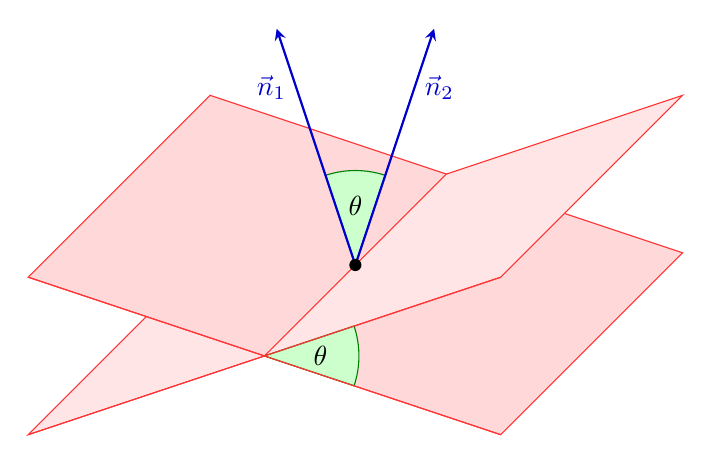
\begin{tikzpicture}
      \filldraw[draw=red!80,fill=red!10] (-3,-1,-3) -- (0,0,-3) -- (0,0,3) -- (-3,-1,3) -- cycle;
      \filldraw[draw=red!80,fill=red!15] (-3,1,-3) -- (3,-1,-3) -- (3,-1,3) -- (-3,1,3) -- cycle;
      \filldraw[draw=red!80,fill=red!10] (0,0,-3) -- (3,1,-3) -- (3,1,3) -- (0,0,3) -- cycle;
      \filldraw[fill=green!20,draw=green!50!black] (0,0,3) -- +(-18.4:12mm) arc (-18.4:18.4:12mm) -- cycle;
      \filldraw[fill=green!20,draw=green!50!black] (0,0,0) -- +(71.6:12mm) arc (71.6:108.4:12mm) -- cycle;
      \draw[red!80] (3,1,3) -- (-3,-1,3);
      \draw[red!80] (3,-1,3) -- (-3,1,3);
      \draw[->,thick,blue!80!black](0,0,0) -- node[left, near end] {$\vect{n}_1$} (-1,3,0);
      \draw[->,thick,blue!80!black](0,0,0) -- node[right, near end] {$\vect{n}_2$} (1,3,0);
      \fill (0,0,0) circle [radius=2.2pt];
      \node at (0,0,0) [above=5mm] {$\theta$};
      \node at (0,0,3) [right=5mm] {$\theta$};
    \end{tikzpicture}
  \end{center}
  The normal vectors are $\vect{n}_1 = \startmat{c}7,-1,0\stopmat^T$ and $\vect{n}_2
  = \startmat{c}4,3,5\stopmat^T$. The angle between them is given by
    \begin{equation*}
    \cos\theta =
    \frac{\vect{n}_1\dotprod\vect{n}_2}{\norm{\vect{n}_1}\norm{\vect{n}_2}}
    = \frac{25}{50} = \frac{1}{2}.
  \end{equation*}
  Therefore, the angle is $\arccos(\frac{1}{2}) = \pi/3$, or 60 degrees.
\end{solution}

\begin{example}{Find the angle between a line and a plane}{angle-line-plane}
  Find the angle between the line
  \begin{equation*}
    \startmat{r} x \\ y \\ z \stopmat
    = \startmat{r} 1 \\ 2 \\ 0 \stopmat
    + t \startmat{r} 2 \\ -1 \\ -2 \stopmat
  \end{equation*}
  and the plane $2x+2y-z = 2$.%
  \index{angle!between line and plane}
\end{example}

\begin{solution}
  To get the angle $\theta$ between the plane and the line, we can
  compute the angle $\phi$ between the direction vector of the line
  and the normal vector of the plane, and then take
  $\theta = \frac{\pi}{2}-\phi$.
  \begin{center}
    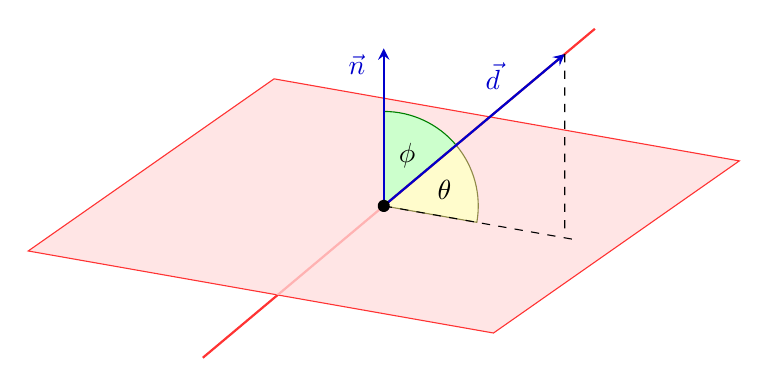
\begin{tikzpicture}[rotate=-10]
      \draw[thick, red!80] (50:-3) -- (0,0);
      \filldraw[draw=red!80,fill=red!10](-3,0,-3.5) -- (3,0,-3.5) -- (3,0,3.5) -- (-3,0,3.5) -- cycle;
      \filldraw[fill=yellow!20,draw=yellow!50!black] (0,0) -- (0:12mm) arc (0:50:12mm) -- cycle;
      \filldraw[fill=green!20,draw=green!50!black] (0,0) -- (50:12mm) arc (50:100:12mm) -- cycle;
      \draw[thick, red!80] (0,0) -- (50:3.5);
      \begin{scope}
        \clip (-3,0,-3.5) -- (3,0,-3.5) -- (3,0,3.5) -- (-3,0,3.5) -- cycle;
        \draw[thick, red!30] (50:-3) -- (0,0);
      \end{scope}
      \draw[->,thick,blue!80!black](0,0,0) -- node[left=3pt, pos=0.9] {$\vect{n}$} (100:2);
      \draw[->,thick,blue!80!black](0,0) -- node[above left, pos=0.7] {$\vect{d}$} (50:3);
      \draw[dashed] (0,0,0) -- (2.5,0,0);
      \draw[dashed] (50:3) -- +(100:-2.3);
      \fill (0,0,0) circle [radius=2.2pt];
      \node at (25:8mm) {$\theta$};
      \node at (75:7mm) {$\phi$};
    \end{tikzpicture}
  \end{center}
  The direction vector of the line is $\startmat{c}2,-1,-2\stopmat^T$ and the normal
  vector of the plane is $\startmat{c}2,2,-1\stopmat$. We have
  \begin{equation*}
    \cos\phi =
    \frac{\vect{n}\dotprod\vect{d}}{\norm{\vect{n}}\norm{\vect{d}}}
    = \frac{4}{9},
  \end{equation*}
  and therefore $\phi = \arccos(\frac{4}{9}) \approx 1.11$ radians. We
  have $\theta = \frac{\pi}{2} - \phi \approx 0.46$ radians, or about
  26.4 degrees.
\end{solution}

\begin{example}{Shortest distance from a point to a plane}{shortest-distance-plane}
  Find the shortest distance from the point $P = (3,2,3)$ to the plane
  given by $2x + y + 2z = 2$, and find the point $Q$ on the plane that
  is closest to $P$.%
  \index{distance!point to plane}%
  \index{projection!point to plane}
\end{example}

\begin{solution}
  In this problem, we are going to use the projection of one vector
  onto another, which was introduced in
  Section~\ref{ssec:projections}.  Pick an arbitrary point $R$ on
  the plane. Then, it follows that
  \begin{equation*}
    \longvect{QP} = \proj_{\vect{n}}\,\longvect{RP}
  \end{equation*}
  and $\norm{\longvect{QP}}$ is the shortest distance from $P$ to the
  plane. Further, the position vector of the point $Q$ can be computed
  as $\vect{q} = \vect{p} - \longvect{QP}$, where $\vect{p}$ is the
  position vector of $P$.
  \begin{center}
    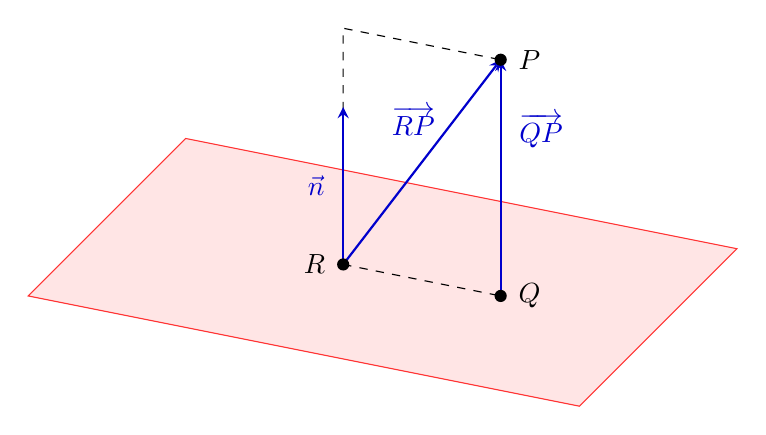
\begin{tikzpicture}[x={(1cm,-0.2cm)},y={(0.5cm,0.5cm)},z={(0cm,1cm)}]
      \filldraw[draw=red!80,fill=red!10](-3,-2,0) -- (4,-2,0) -- (4,2,0) -- (-3,2,0) -- cycle;
      \draw[dashed](0,0,0) -- (2,0,0) -- (2,0,3) -- (0,0,3) -- cycle;
      \draw[->,thick,blue!80!black](0,0,0) -- node[left=3pt] {$\vect{n}$} (0,0,2);
      \draw[->,thick,blue!80!black](0,0,0) -- node[left=3pt, pos=0.7] {$\longvect{RP}$} (2,0,3);
      \draw[->,thick,blue!80!black](2,0,0) -- node[right=3pt, pos=0.7] {$\longvect{QP}$} (2,0,3);
      \fill (0,0,0) circle [radius=2.2pt] node [left=3pt] {$R$};
      \fill (2,0,3) circle [radius=2.2pt] node [right=3pt] {$P$};
      \fill (2,0,0) circle [radius=2.2pt] node [right=3pt] {$Q$};
    \end{tikzpicture}
  \end{center}
  From the above scalar equation, we have that $\vect{n} =
  \startmat{c} 2 \\ 1 \\ 2 \stopmat$.  Now, choose any
  point on the plane, for example, $R = (1,0,0)$ (notice that this
  satisfies $2x+y+2z=2$).  Then,
  \begin{equation*}
    \longvect{RP} = \startmat{c} 3 \\ 2 \\ 3 \stopmat
    - \startmat{c} 1 \\ 0 \\ 0 \stopmat =
    \startmat{c} 2 \\ 2 \\ 3 \stopmat.
  \end{equation*}
  Next, compute $\longvect{QP} = \proj_{\vect{n}}\longvect{RP}$.
  \begin{equation*}
    \longvect{QP} ~=~ \proj_{\vect{n}}\longvect{RP}
    ~=~ \paren{\frac{\vect{n}\dotprod\longvect{RP}}{\norm{\vect{n}}^2}}\vect{n}
    ~=~ \frac{12}{9} \startmat{r} 2 \\ 1 \\ 2 \stopmat
    ~=~ \frac{4}{3} \startmat{r} 2 \\ 1 \\ 2 \stopmat.
  \end{equation*}
  Then, $\norm{\longvect{QP}} = 4$ so the shortest distance from $P$
  to the plane is $4$.  To find the point $Q$ on the plane that is
  closest to $P$, we have
  \begin{equation*}
    \vect{q} ~=~ \vect{p} - \longvect{QP}
    ~=~ \startmat{r} 3 \\ 2 \\ 3 \stopmat
    -
    \frac{4}{3} \startmat{r} 2 \\ 1 \\ 2 \stopmat
    ~=~
    \frac{1}{3}
    \startmat{r} 1 \\ 2 \\ 1 \stopmat.
  \end{equation*}
  Therefore, $Q = (\frac{1}{3},\frac{2}{3},\frac{1}{3})$.
\end{solution}

\end{document}

